\documentclass[10pt,twosides]{report}
\usepackage[english]{babel}


\usepackage{graphicx} 
\usepackage{spverbatim}

\begin{document}
\begin{center}
		\large \textbf{Ahsanullah University of Science and Technology} 
		
		Department of Computer Science and Engineering
		\vspace{0.1in}
	\end{center}
	\begin{center}
		
\includegraphics[scale=0.4]{figures/logo}
	\end{center}
	\begin{center}
		\large \textbf {Car Rent and Sell}
		\vspace{0.3in}
		\\
		Information System Design    
		\\
		and
		\\
		Software Engineering Lab(CSE 3224)
		\vspace{0.3in}
		\\ \textbf{Submitted to }
		\vspace{0.1in}
		\\ \textbf{Mr. Emam Hossain}
		\\ \textbf{Assistant Professor, AUST}
		\vspace{0.1in}
		\\ \textbf{Dr. Nusrat Sharmin, }
		\\ \textbf{Lecturer, AUST}
		\vspace{0.2in}
		\\ \textbf{ Submitted By:}
		\vspace{0.1in}
		\\ {Md. Rubel Mia}
		\\ {ID: 15.02.04.007}
		\\ {Asadullahhil Galib}
		\\ {ID: 15.02.04.022}
		\\ {Narayan Das Nitol}
		\\ {ID: 15.02.04.025}
		
		
	\end{center}
	\pagebreak

\pagenumbering{roman}
 \tableofcontents
 
\listoffigures

\listoftables

\newpage
  \pagenumbering{arabic}             

\setcounter{chapter}{0}
 
 \chapter{Introduction}

\textbf{}\\
We’re living in a world of click-and-consume. All our car customers can buy anything they want online. So, often in the auto industry, we forget that long before they hit the lot, consumers are looking online for their next car. To do that, we have to promote our inventory. As, we start to build our online inventory, think of it more as a front door to our dealership. We are welcoming people . We are showing them around. We are making them feel comfortable with our inventory. Our online inventory is a way for people to collect leads which is just one of many ways to rent and sell cars online. \\



\noindent 

\noindent 
\section{   Project Goal}

\noindent 



\begin{enumerate}
\item         It will optimize the time spend in the activities performed during the sale and rent purposes.

\item 	It will help customers to choose their dream car sitting at their home.

\item 	It will gain maximum business region.

\item        Providing better accessibility and up to date information for customer.

\item        Managing important data and information of car and customer and place.

\item	       Providing a friendly interface for the customer/tourist.
\end{enumerate}

\noindent 

\noindent 

\noindent 

\noindent 

\noindent 

\noindent 

\noindent 


\newpage


\section{   Features}

\noindent 


\begin{enumerate}
\item         The main purpose of Car Rent and Sell is buy and rent cars online. Using this project anyone can rent/buy cars online including by budget, cities, model, company etc.

\item 	Our project is meant to give people a better and trustworthy platform where they can buy and rent cars of their own choice and obviously on their own terms and condition.

\item 	With the help of internet and computer systems a man from remote area can buy his car from anywhere the country/world.

\item        This project will provide facility to all buyer, seller and dealers for rent/sell cars. If anyone want to buy cars online, then first he will register in this website and then he can see all the details about the cars including prices, model and features.

\item        Any person can register in the website and after that he can buy and rent cars, compare the cars regarding budget, model, company, city. Unregistered person may only see common pages with all buyer and seller’s information.
\end{enumerate}

\noindent 

\noindent 

\noindent 

\noindent 

\noindent 




\section{    Feasibility Analysis}

\noindent Feasibility Analysis lets the developer foresee the future of the project and the usefulness. Feasibility Analysis of a system or website is according to its workability, ability to meet their user needs and effective use of resources. Thus when a new application is proposed it normally goes through a feasibility study. Here we are going to provide the feasibility of the project that is being designed and lists various areas that will be considered very carefully during the feasibility study of our website such as Technical, Economical and Operational feasibilities.
\noindent 

\newpage
\subsection{    Technical Feasibility }
The website must be evaluated from the technical point of view first. The assessment of this feasibility must be based on an outline design of the system requirement in the terms of input, output, programs and procedures. This website will be done with following elements given below :
\noindent 

\begin{enumerate}
\item  \textbf{Front-end Language:} HTML, CSS

\item  \textbf{Back-end Language:} ASP.NET
\\
\end{enumerate}



\subsection{    Economical Feasibility } 

Economical feasibility is the second part of resource determination. This includes the time of the system analysis team, the cost of doing a full systems study (including the time of employees) the cost of the business employee time, the estimated cost of hardware/software or software development. Developing this application is highly economically feasible. We don’t need to spend much money for the development of the system. The only thing to development with an effective supervision. The costs for the software developers and servers are reasonable and the company for which the project will be developed will be highly benefited by serving customers as well as selling auto parts as every details of the servicing and selling of parts will be listed in the system. So, we can say that our project is economically feasible.

\noindent 
\paragraph{}




\begin{table}

\subsection{   Operational Feasibility }
The system analyst must consider the operational feasibility of the requested project even if the technical and economic resources are both judged adequate. Operational feasibility is dependent on the human resources available for the project and involves projecting whether the system will operate and be used once it is installed. If users are virtually used to the present system, see no problems with it and generally are not involved in requesting a new system, resistance to implementing the new system will be strong. Chances for it ever becoming operational are low. Alternatively, if users themselves have expressed a need for a system that is operational more of the time, in a more efficient and accessible manner, chances are better that the requested system will eventually be used.  



\section{   Cost and Benefit Analysis}

Cost Benefit Analysis estimates and totals up the equivalent money value of the benefits and costs to the community of projects to establish whether they are worthwhile. Tangible and Intangible are the types of Cost Benefit Analysis.  The Cost Benefit Analysis of our project is given below:\\

\includegraphics*[width=5.3in, height=3in, keepaspectratio=false]{figures/CostBenifit}

\caption{Cost Benefit Analysis for Car Rent and Sell Website}

\end{table}



\begin{table}
\subsection{    Cash Flow Analysis}
\noindent An examination of a company's cash inflows and outflows during a specific period. The analysis begins with a starting balance and generates an ending balance after accounting for all cash receipts and paid expenses during the period. The cash flow analysis is often used for financial reporting purposes. See also cash flow projection, cash flow forecast:\\


\includegraphics*[width=5.51in,height=3in]{figures/CashFlow}
\caption{Cash Flow Analysis for Car Rent and Sell Website} 
 
\subsection{    Present Value Analysis}

\noindent Present value (PV) is the current value of a future sum of money or stream of cash flows given a specified rate of return. Future cash flows are discounted at the discount rate, and the higher the discount rate, the lower the present value of the future cash flows. Determining the appropriate discount rate is the key to properly valuing future cash flows, whether they be earnings or obligations.

\noindent \includegraphics*[width=5.71in, height=2.4in]{figures/PV}

\end{table}



\noindent 

\begin{table}
\section{   Project Scheduling}
Project scheduling is a mechanism to communicate what tasks need to get done and which organizational resources will be allocated to complete those tasks in what timeframe. A project schedule is a document collecting all the work needed to deliver the project on time. The table is given below:\\


\noindent \includegraphics*[width=5.3in, height=3 in]{figures/PS}

\caption{Project Scheduling for Car Rent and Sell Website}

\end{table}

\begin{figure}

\subsection{   Gantt Chart}
A Gantt chart, commonly used in project management, is one of the most popular and useful ways of showing activities (tasks or events) displayed against time. On the left of the chart is a list of the activities and along the top is a suitable time scale. Each activity is represented by a bar; the position and length of the bar reflects the start date, duration and end date of the activity. The gantt chart of our project is given below:\\\\


\noindent \includegraphics*[width=5.51in, height=3 in]{figures/gannt_chart}

\caption{Gantt Chart for Car Rent and Sell Website}


\noindent 

\noindent 
\section{  Conclusion}

We know about that people in our country, who want to buy a new car, must have to go first in the car showroom., then choose his/her cars, then purchase it. This process is very time consuming. So, our main goal is to reduce the time-consuming factors.
\noindent 
\end{figure}
\noindent 


\chapter{Information Gathering}

\noindent 
\paragraph{\Large Introduction }\textbf{}\\~~We know about that people in our country, who want to buy a new car, must have to go first in the car showroom., then choose his/her cars, then purchase it. This process is very time consuming. So, our main goal is to reduce the time-consuming factors. For making our project successful, we need to follow some steps gradually for the entire development of this project. Regarding this, information gathering is the first and foremost step. \\


\noindent 

\noindent 
\section{ Objectives of Information Gathering  \&  \newline Interview}

\noindent The name of our project is CAR Rent \& Sell. To make the project user-friendly, by useful data and information, it is important to interview authority of the car showroom. The information obtained from the relevant people working there would help us for the project to be perfect and precise work. Here we have constructed interview questions to gather information requirements and structured them in a meaningful way. All this information is gathered from the authority who invoked us to work for this project. According to the gathered information and collection of data, we have numerous scopes to improve the features and add new functionalities in future.


\noindent 

\noindent 

\noindent 
\section{ Questionnaire \& Interview Pattern}

\noindent Interviewing is a specific form of meeting or conference, and is usually limited to two persons, the interviewer and the interviewee. We have assembled information using the following 1 methods:

\begin{enumerate}
\item  \textbf{Interview of the authority :}We interviewed Mr. Tanvir Ahmed Iftekhar who is the Sales Executive of the Navana Limited.

\end{enumerate}

\noindent For both methods of question and answers, we have chosen \textbf{Diamond shaped Structure}. The diamond-shaped structure for interviewing combines the pyramid and funnel structure. This structure entails beginning in a very specific way, then examining general issues, and finally coming to a very specific conclusion. So, we decided to work with this structure.  

\noindent In the interview process, we have included:

\begin{enumerate}
\item  4 Close Ended questions at first. 

\item  4 Open Ended questions in the middle

\item  2 Close Ended questions at last
\end{enumerate}
\noindent The table pattern for interview \& questionnaire is given below:

\begin{table}



\begin{tabular}{|p{1.3in}|p{1in}|p{1.1in}|p{1.1in}|} \hline 
\multicolumn{4}{|p{5in}|}{\textbf{~~~~~~~~
~~~~~~~~~Car Rent and Sell Website}} \\ \hline 
\textbf{Authors:\newline \newline }Md.~Rubel~Mia\newline Asadullahhil~Galib\newline Narayan~Das~Nitol\textbf{} & \textbf{Date:\newline \newline }23-05-2018 & \textbf{Time:\newline \newline }02:30 pm \textbf{} & \textbf{Duration:\newline \newline }\newline 60mins \textbf{} \\ \hline 
\multicolumn{2}{|p{2in}|}{\textbf{Participants:\newline  }Mr. Tanvir Ahmed Iftekhar\textbf{\newline }Sales Executive – Navana Limited \newline } & \multicolumn{2}{|p{2.4in}|}{\textbf{Comments:\newline }\newline We have got a clear idea of the website that authority requires and the current existing systems \newline } \\ \hline 
\end{tabular}

\caption{ Interview  Questionnaire Pattern of Car Rent \& Sell Website}

\end{table}

\noindent 
\section{ Reason To Select Interview Personnel}

\noindent As Mr. Tanvir Ahmed Iftekhar is the Sales Executive of Navana Limited, he has the utmost knowledge of which is required for his company to flourish further. He knows better about entire sector of this company. That’s why we have selected for the interview.

\noindent \\


\noindent 

\newpage 

\subsection{ Interview Questions \& Answers }
\begin{enumerate}
    \item \textbf{How many people are working in this showroom?}
    \noindent \textbf{\underbar{Answer:}}65.
    
    \item \textbf{How many people are working in this showroom?}\newline
    \noindent \textbf{\underbar{Answer:}}Around 500.
    
     \item \textbf{Do you have any existing website for your company?}\newline
    \noindent \textbf{\underbar{Answer:}}Yes. It is www.amartoyota.com.
    
    \item \textbf{Do you want any online customer support?}\newline
    \noindent \textbf{\underbar{Answer:}}Yes. 
    
    \item \textbf{How many cars you are selling in a month?}\newline
    \noindent \textbf{\underbar{Answer:}}Well, its very tough to say. Because it is not constant. It varies from month to month. As an example, sometimes we sell around 5 cars in a month. And sometimes we sell around 100 cars in a month. In the month of May-July, we sell maximum cars as it is the month of Government Purchase. Government alone buys maximum car for their employee and higher authority.

    
    \item \textbf{How many categories you want to include in this website?}\newline
    \noindent \textbf{\underbar{Answer:}} There should be 5 categories in the website :\newline
	\begin{enumerate}
		\item Choice
		\item Test Drive
		\item Verification
		\item Rent a Car
		\item Services
	\end{enumerate}
    
   
    \item \textbf{Do you want to include any virtual reality system in this website?}\newline
    \noindent \textbf{\underbar{Answer:}} Obviously. I want a 3D view of our showroom where people can see like the real one. Our customer can get the real feel of our showroom seating at their house. Customers can open the door of a car virtually, can see the windshield virtually, also can drive the card virtually. This will help our customers to select their cars.
    
    \item \textbf{How you will control the Car Rental System of this website?}\newline
    \noindent \textbf{\underbar{Answer:}}Those cars which we want to rent, there will be a GPS system included with every cars. We can track any cars as we want. So, our cars will remain safe. We will provide 2 packages for our clients for rental purpose :
	\begin{enumerate}
		\item Car with Driver
		\item Car without Driver		
	\end{enumerate}
	\noindent Car with a driver - in this package, our official driver will drive the cars \newline
	Car without driver - in this package, our clients will drive the cars.

    
    \item \textbf{Which things is the must you want to include in the website?}\newline
    \noindent \textbf{\underbar{Answer:}}A realistic picture of the car with the price tag.  
    
    \item \textbf{Do you want any online review system for every car in your showroom?}\newline
    \noindent \textbf{\underbar{Answer:}}Yes. We will upload every video of every single cars of your showroom so that our customer will get a clear idea.
    
    \end{enumerate}

\section{Revised Requirement Analysis}

\noindent Through all the information collection, we revised our work and concluded that along with our features. For this constant update of information, we will need to create an Virtual Reality System. This will remain in our future goal for this application.

\begin{enumerate}
\item  User friendly interface.

\item  Well-interactive interface between customer and employee.

\item  Adding a searchbox for initial search.

\item  Admin panel is a must for handling the dealer, product and employee.

\end{enumerate}

\noindent 

\noindent 
\section{ The list of Activities}

\noindent We have interviewed people of a company before designing the project. We have collected the following information:

\begin{enumerate}
\item  How the services are provided to the customers.

\item  How the services are provided to the customers.

\item  How they will manage the entire system.

\item  The security management of the rental cars.

\item  Virtual Reality of the showroom.

\end{enumerate}

\noindent 
\noindent
We also wanted to know the problems they are encountering for not having any dynamic website. We gathered the critical information from them regarding the types of features they want in the website. All these data and information would help us to design the website.

\noindent 
\noindent

\section{ Conclusion}

\noindent The interview and survey process gave us the opportunity to visit and interview different people and helped us a lot to know what users actually want from a website which contains information of such things related to buy rent a car company. These information and data will help us to design a website according to user choice and make our work easier

\noindent 

\noindent 

\noindent 

\noindent 



\chapter{Data Flow Diagram and Use Case Diagram}

\noindent 
\paragraph{\Large{Introduction}}

\noindent\\ \textbf{ Data Flow Diagram (DFD)} graphically representing the functions, or processes, which capture, manipulate, store, and distribute data between a system and its environment and between components of a system. The visual representation makes it a good communication tool between User and System designer. Structure of DFD allows starting from a broad overview and expand it to a hierarchy of detailed diagrams. DFD has often been used due to the following reasons:
\noindent 

\begin{enumerate}
\item  Logical information flow of the system.

\item  Determination of physical system construction requirements.

\item  Simplicity of notation.

\item  Establishment of manual and automated systems requirements.
\end{enumerate}

\noindent 
\section{Activities of the project}

\noindent The activities of our project are given below:

\begin{enumerate}
\item  Ensure user-friendly interface.

\item  Creating search field.

\item  Creating compare field.

\item  Add review.

\item  Choose cars.

\item  Creating an advance database for rental cars.

\item  Test-drive scheduling.

\item  Rental car scheduling.

\end{enumerate}

\noindent 

\noindent 

\noindent 

\section{Main Process}

\noindent There are 5 main process in our system:

\begin{enumerate}
\item  Select Car.

\item  Registration for order

\item  Cancel order.

\item  Update order.

\item  Review.

\end{enumerate}

\noindent 
\section{Sub Processes}

\noindent There are 3 sub processes under \textbf{Select Car}

\begin{enumerate}
\item  Display Car

\item  Check Availability

\item  Search Car.

\end{enumerate}

\noindent 

\noindent There are 2 sub processes under \textbf{Registration for order}

\begin{enumerate}
\item  Register for Test drive 

\item  Register for Rent


\end{enumerate}

\noindent 

\noindent There are 1 sub processes under \textbf{Cancel Order}

\begin{enumerate}
\item  Cancel Order

\end{enumerate}

\noindent 

\noindent There are 1 sub processes under \textbf{Update Product}

\begin{enumerate}
\item  Update Product

\end{enumerate}

\noindent 

\noindent There are 1 sub processes under \textbf{Product Review}

\begin{enumerate}
\item  Product Review

\end{enumerate}

\noindent 





\section{Entity Names}

\noindent There are total 2 entity in our system:

\begin{enumerate}
\item  Customer

\item  Admin
\end{enumerate}

\noindent 
\section{Database Names}

\noindent There are total 5 table in our system Database:

\begin{enumerate}
\item  Car info

\item  Order info

\item  TestDrive info

\item  Rent info

\item  Review


\end{enumerate}


\noindent 

\section{Data Flow Diagram Levels}

\noindent A data flow diagram can dive into progressively more detail by using levels and layers. The first level of DFD shows the main process within the system. This main process can be divided into further processes until we reach the final level. DFD levels are numbered 0, 1 or 2, and occasionally can go to even Level 3 or beyond. All these levels define the scope of what we are trying to accomplish. For our project we have constructed 3 levels. The levels are given below:

\begin{enumerate}
\item  Context Level/ Level 0

\item  Level 1

\item  Level 2
\end{enumerate}

\noindent 



\section{Context Level Diagram}

\noindent Context Diagram is a basic overview of the whole system or process being analyzed or modeled. It’s designed to be an at-a-glance view, showing the system as a single high-level process, with its relationship to external entities. It only contains one process node that generalizes the function of the entire system in relationship to external entities.


\begin{figure}
\noindent The diagram of the Context Level of our project is given below:\\



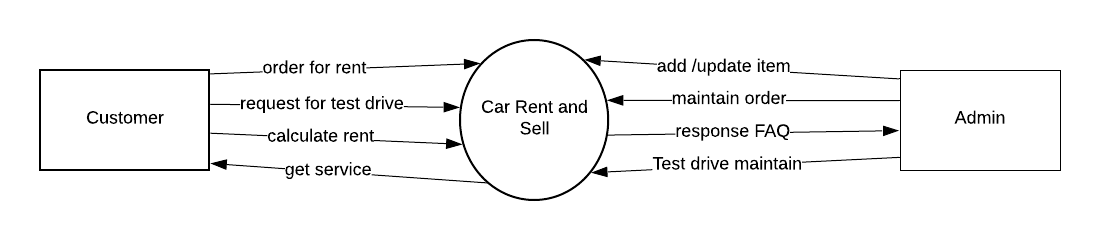
\includegraphics[width=6.00in, height=5.50in]{figures/C0}

\noindent 

\noindent 
{\bf Figure 3.1: Context Level diagram of Car Rent and Sell Website}
\end{figure}

\noindent 

\begin{figure}


\section{Level 1 Diagram}

\noindent A level 1 data flow diagram (DFD) is more detailed than a level 0 DFD but not as detailed as a level 2 DFD. It breaks down the main processes into subprocesses that can be analyzed and improved on a more intimate level.

\noindent The diagram of Level 1 is given below:\\


\noindent 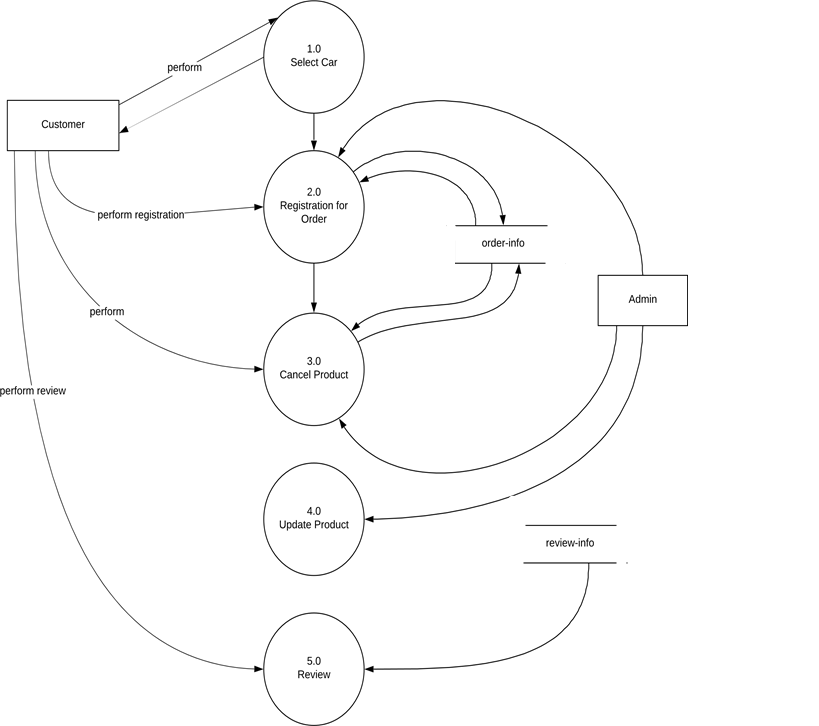
\includegraphics[width=5.50in, height=7.21in, keepaspectratio=false]{figures/C1}

\noindent 

\caption{Level 1 diagram of Car Rent and Sell Website}


\end{figure}


\noindent 
\begin{figure}


\section{Level 2 Diagram}

\noindent A level 2 data flow diagram (DFD) offers a more detailed look at the processes that make up an information system than a level 1 DFD does. It can be used to plan or record the specific makeup of a system.

\noindent \\


\textbf{1.Select Car Process:}


\noindent \textbf{}

\noindent 

\noindent The diagram of Select Car Process is given below:

\noindent 

\noindent \includegraphics*[width=5.70in, height=3.17in, keepaspectratio=false]{figures/SelectCar}

\noindent 

\caption{Select Car Process of Car Rent and Sell Website}
\end{figure}
\noindent 

\noindent 

\noindent 
\begin{figure}



 \textbf{2.Registration for Order Process:}


\noindent 

\noindent The diagram of Registration for Order Process of Car Rent and Sell Website is given below:

\noindent 

\noindent \includegraphics*[width=6.50in, height=3.50in, keepaspectratio=false]{figures/Registration}
\caption{Registration for Car Process of Car Rent and Sell Website}
\end{figure}
\noindent 

\noindent 

\noindent 

\noindent 

\noindent 

\noindent 
\begin{figure}


 \textbf{3.Cancel Order Process:}


\noindent 

\noindent 

\noindent The diagram of Cancel Order Process of Car Rent and Sell Website is given below:

\noindent 

\noindent \includegraphics*[width=6.50in, height=3.33in, keepaspectratio=false]{figures/Cancel}
\caption{ Cancel Order Process of Car Rent and Sell Website}
\end{figure}
\noindent 

\noindent 
\begin{figure}


 \textbf{4.Update Order Process}


\noindent 

\noindent 

\noindent 

\noindent The diagram of Update Order Process of Car Rent and Sell Website is given below:

\noindent 

\noindent \includegraphics*[width=5.50in, height=3in, keepaspectratio=false]{figures/Update}

\caption{Update Order Process of Car Rent and Sell Website}
\end{figure}
\noindent 

\noindent 
\begin{figure}

 \textbf{5.Review}


\noindent 

\noindent The diagram of Review Process of Car Rent and Sell Website is given below:

\noindent \includegraphics*[width=5.50in, height=3in, keepaspectratio=false]{figures/Review}

\caption{ Review Process of Car Rent and Sell Website}
\end{figure}
\noindent 

\noindent 

\noindent 


\begin{figure}

\section{Use Case Diagram}

\noindent A Use Case model defines what a system does without describing how the system does it. This logical model of the system replicates the understanding of a system from the viewpoint of a user outside the system, which is the system's requirement. It also splits the mode of the system that works into actions, services and reactions that are major to the users of the system.


\subsection{Actors}

\textbf{Customer: }Customers can select car, ask for test drive, rent car, cancel orders.\newline
\textbf{Admin: }Admin can manage registration process, update products and make orders decisions.

\subsection{Details of Use Case Models}

\noindent In Car Rent and Sell Website, we have the following use cases for these two actors:

\noindent \textbf{\underbar {Select Car}}

\noindent Actor: Customer
\noindent Primary Path:

\begin{enumerate}
\item  Check availability.

\item  Select required car. 
\end{enumerate}

\noindent \textbf{\underbar {Registration for Order}}

\noindent Actor: Customer
\noindent Primary Path:

\begin{enumerate}
\item  Collect customer’s info.

\item  Verify customer. 
\end{enumerate}

\noindent Alternative Path:
\begin{enumerate}
\item  In case of failure display registration error.

\end{enumerate}

\noindent \textbf{\underbar {Cancel Order}}

\noindent Actor: Customer
\noindent Primary Path:

\begin{enumerate}
\item  Confirm Cancellation

\end{enumerate}


\noindent \textbf{\underbar {Update Product}}

\noindent Actor: Admin
\noindent Primary Path:

\begin{enumerate}
\item  Add new car.

\item  Remove unavailable car.

\item  Update rent price and selling price.
\end{enumerate}


\noindent Alternative Path:
\begin{enumerate}
\item  Can’t update due to some unexpected reason.

\end{enumerate}


\noindent \textbf{\underbar {Review}}

\noindent Actor: Customer
\noindent Primary Path:

\begin{enumerate}
\item  Can review rent service.

\item  Can review sell service.

\end{enumerate}

\end{figure}

\begin{figure}

\subsection*{Use Case Relationships}

\noindent The final element in Use Case diagrams are Relationships. There are 4 types of relationships:

\noindent 
\subsection{Association}

\noindent An association between an actor and a use case specifies that the actor and the use case in some way interact or communicate with each other. In this relationship, an actor is connected to a use case using line with no arrowheads.


\noindent 
\subsection{Include}

\noindent Between 2 use cases include is a directed relationship, used to show that performance of the included use case is inserted into the behavior of the including (base) use case. Usually a use case comprises a behavior that is common to more than one other use case. Here, the arrow directs to the common use case.


\subsection{Extend}

\noindent Extend identifies how \& when the behavior cleared in usually optional extending use case can be introduced into the behavior established in the extended use case. From the base use case, different use cases handle exceptions. The arrow plugs from the extended to the base use case.\textbf{}
\end{figure}
\begin{figure}

\noindent 
\subsection{Generalization/ Inheritance}

\noindent Generalization states the relationship that can happen between two use cases and shows that one use case (child case) inherits the structure, behavior and relationships of the another actor (parent). Here, the arrow points to the general use case (parent case).


\noindent 
\subsection*{Extension Points}

\noindent Use cases can include conditional steps as well as extensions or alternative scenarios. Extension point is a property of a use case that categorizes a point where the actions of a use case can be amplified with elements of another (extending) use case.



\noindent 


\section{Use Case Models}


\noindent \includegraphics*[width=5.51in, height=4 in]{figures/use}

\caption{Use Case Diagram for Car Rent and Sell Website}


\section{Conclusion}

\noindent As our project is Car Rent and Sell, the main intention behind this project is to provide such type of facilities which can prevent the wastage of time while buying car in the showroom and book a car for rental purpose. With the help of data flow diagram, we have achieved the clear idea about process on the system and relations among them. In use case diagram we have found the relationship among actors and entire system which will help to develop our project very clearly and smoothly.

\end{figure}
\chapter{Relationship Diagram and Class Diagram}
 
\noindent 
\paragraph{Introduction}

\noindent \textbf{Class diagram} and \textbf{Entity Relationship Diagram(ERD)} both model is the structure of a system. \textbf{Class diagram} represent the dynamic aspects of a system, both the structural and behavioral features. \textbf{ERD} represents only structural features which provide a static view of the system.


\noindent 

\noindent 


\section{ Entity Relationship Diagram (ERD)}

\noindent An entity relationship model, also called an \textbf{Entity Relationship Diagram (ERD)} is a graphical representation of entities and their relationships to each other, typically used in computing in regard to the organization of data within databases or information systems. An \textbf{Entity Relationship Diagram (ERD)} shows the relationships of entity sets stored in a database. An entity in this context is a component of data. In other words, ER diagrams illustrate the logical structure of databases.

\noindent A basic ER model is composed of entity types and specifies relationships that can exist between instances of those entity types. The 3 key components of ERD are:

\begin{enumerate}
\item  Entity

\item  Relationship

\item  Attribute
\end{enumerate}

\begin{figure}

\subsection{ ER Diagram}

\includegraphics*[width=6.3in, height=3in, keepaspectratio=false]{figures/erd}

\caption{ER Diagram for Car Rent and Sell Website}

\end{figure}



\noindent 
\subsection{ Entities}

\noindent Entity will be real world object from problem domain and data will be stored in the database on entity. It is noun all time and distinguishable from other objects.

\noindent In our project, we have the following entities in the ERD:

\begin{enumerate}
\item  Customer

\item  Admin

\item  Rent\_Car

\item  Test\_Drive

\item  Gallery

\end{enumerate}

\noindent 

\noindent 

\noindent 
\newpage

\subsection{ Relationships}

\noindent The interaction between the entity set are called relationship. It is always a verb and creates association among two or more attributes.

\noindent In our project, the relationships between the entity sets are:

\noindent \textbf{Entity Set 1:} Customer, Rent\_Car

\noindent \textbf{Relationship:} Order

\noindent 

\noindent \textbf{Entity Set 2:} Admin, Rent\_Car

\noindent \textbf{Relationship:} Approve

\noindent 

\noindent \textbf{Entity Set 3:} Customer, Text\_Drive

\noindent \textbf{Relationship:} Request

\noindent 

\noindent \textbf{Entity Set 4:} Admin, Text\_Drive

\noindent \textbf{Relationship:} Arrange

\noindent \textbf{Entity Set 5:} Admin, Gallery

\noindent \textbf{Relationship:} ManagedBy

\noindent 

\noindent 
\subsection{ Cardinality Constraints of Relationship}

\noindent The maximum number of entity that can be associated with another entity via a relationship, are defined as cardinality ratio. It is most useful in describing binary sets of relationship sets. There are 4 types of cardinality constraints:

\begin{enumerate}
\item  Many to many

\item  Many to one

\item  One to many

\item  One to one
\end{enumerate}


\noindent 


\noindent 

\subsection{ Attributes}

\noindent The properties of entity or relationship are called attributes. An entity is basically described using a set of attributes. In our project, we have the following attributes of each entity in the ERD:

\noindent \textbf{Entity Name: } Customer

\noindent \textbf{Attributes:}

\begin{enumerate}
\item user\_id

\item  name

\item  email

\item  password

\item  address

\item  nid
\end{enumerate}

\noindent

\noindent \textbf{Entity Name: } Rent\_Car

\noindent \textbf{Attributes:}

\begin{enumerate}
\item rent\_car\_id

\item  car\_model

\item  time\_period

\item  date\_time

\item  no\_of\_cars

\end{enumerate}

\noindent

\noindent \textbf{Entity Name: } Admin

\noindent \textbf{Attributes:}

\begin{enumerate}
\item admin \_id

\item  password

\item  email

\item  address

\item  phone

\item  mobile

\end{enumerate}

\noindent

\noindent \textbf{Entity Name: } Test\_Drive

\noindent \textbf{Attributes:}

\begin{enumerate}
\item car\_id

\item  user\_id

\item  date\_time

\item  car\_model

\end{enumerate}

\noindent

\noindent \textbf{Entity Name: } Gallery

\noindent \textbf{Attributes:}

\begin{enumerate}
\item car\_id

\item  car\_model

\item  car\_type

\item  car\_company

\item  price
\end{enumerate}




\noindent 

\noindent 



 
\section{ Class Diagram}

\noindent Class diagrams are fundamental to the object modeling process and model the static structure of a system. Class diagrams is a snapshot that describes exactly how the system works, the relationships between system components at many levels, and how to implement those components.

\noindent During the analysis and design phases of the development cycle, create class diagrams to perform the following functions:

\begin{enumerate}
\item  Define the structure of classes and other classifiers.
\item  Define relationships between classes and classifiers.
\item  Illustrate the structure of a model by using attributes, operations, and signals.
\item  Show the common classifier roles and responsibilities that define the behavior of the system.
\item  Show the implementation classes in a package.
\item  Show the structure and behavior of one or more classes.
\end{enumerate}

\noindent 

\subsection{Classification}
\noindent Class Diagram has three parts:
\begin{enumerate}
\item  Class
\item  Attribute
\item  Method
\end{enumerate}

\noindent 
\noindent  \textbf{1. Class}
\noindent Classes represent an abstraction of entities with common characteristics.
\noindent  \textbf{2. Attribute}
\noindent An attribute is a named property of a class that describes the object being model. In class diagram, attributes appear in the second compartment just below the name compartment.
\noindent  \textbf{3. Method}
\noindent Method describe the class behavior and appear in the third compartment.


\noindent 
\subsection{Relationship}

\noindent There are 4 types of relationships in a class diagram:

\noindent 
\subsubsection{ Inheritance}

\noindent Inheritance refers to the ability of one class (child class) to~inherit~the identical functionality of another class (parent class), and then add new functionality of its own. The advantage of inheritance is if we want to add or change attributes of the child classes, we don't have to change the subclasses, we can only change the super class and it applies across all sub classes.


\noindent 
\subsubsection{ Association}

\noindent The simplest type of relationship is association, whose presence or absence does not affect in the whole scenario of the class diagram. Associations are shown as a simple line on a class diagram.


\noindent 


\noindent 
\subsubsection{ Aggregation}

\noindent Aggregation offers a means of showing that the whole object is composed of the sum of its parts. It is often described as a ``has'' relationship. The diamond in the end of the relationship line is not filled in here. It is a special type of association that specifies the whole and its parts.


\noindent 


\noindent 
\subsubsection{ Composition}

\noindent Composition is a whole/ part relationship in which the whole has a responsibility for the part, is a stronger relationship. It is usually shown with a filled-in diamond. The classes which are related through composition relationship are dependent on each other.



\noindent

\subsection{ Visibility}
\noindent We use visibility markers to signify who can access the information contained within a class. Private visibility, denoted with a - sign, hides information from anything outside the class partition. Public visibility, denoted with a + sign, allows all other classes to view the marked information. Protected visibility, denoted with a \# sign, allows child classes to access information they inherited from a parent class.

\noindent
\noindent

\subsection{ Classes of our project}
\noindent The class names are listed below:

\begin{enumerate}
\item  Customer
\item  Rent\_Car
\item  Admin
\item  Gallery
\item  Test\_Drive
\item  Review
\end{enumerate}

\noindent

\subsection{ Class Diagram}

\begin{figure}

\noindent The class diagram of Car Rent and Sell Website is given below:

\noindent \includegraphics*[width=5.48in, height=7.2in, keepaspectratio=false]{figures/ClassDiagram}
\caption{Class Diagram Of Car Rent and Sell Website}
\end{figure}
\noindent 


\noindent 
\section{ Conclusion}

\noindent A use case diagram provides project planning skeleton. We have thought through every user’s needs and designed our class diagram. The entity relationship diagram (ERD) is the logical structure of database and shows relationships of entity sets stored in a database. We have illustrated all the entities, attributes, data types and relationships of our entity relationship diagram. Above mentioned diagrams will help us to visualize the whole system more evidently


\noindent 

\noindent 






\chapter{Discussion}

\noindent 

\noindent 
\paragraph{\large{Conclusion}}

\noindent\\ The main focus of Car Rent and Sell website is to consume time of customers to choice cars and also to rent a car for their different purpose. Customers do not need any physical contact of the showroom , rather than they can choose car from anywhere of the country. We have initially started our project by our imagination and the requirements of the company. After that we have gone through all the feasibility analysis, cost benefit analysis, cash flow analysis and so on. We have also designed our Gantt chart and started working by following the project scheduling of our project. Then we interviewed the authority. We also gathered information to know the requirements of the authority.

\noindent After the interview we have designed our Data Flow Diagram (DFD) by which we got the specific vision of our project and got a clear graphical representation of our system's requirements. After designing the DFD, we designed our Use Case Diagram.Then we designed the entity relationship diagram (ERD) which is the logical structure of database and shows relationships of entity sets stored in a database. We have also designed our class diagram which contains all relevant relations and data types.


\noindent 

\noindent 
\section{ Limitation}

\noindent We tried our best to impliment all the features of our project which the authority wants. We have collected every important information about this company which is related to our project. But after all, we have some limitations in our project which we could not impliment at all but have plan to do it in future.

\noindent The limitations of our project are given below:

\begin{enumerate}
\item  We have designed our website only for 1 showroom.

\item  Rental management system is not satisfactory.

\item  Vistual Reality System is not implimented.

\item  Online paylemt is not included in our website.

\item  Online Customer Support feature is not working.
\end{enumerate}

\noindent 

\noindent 
\section{ Future Work}

\noindent In future we will fulfill the limitations of our website which we mentioned before. Then we have also some idea related to Car Rental System which will give customer more pleasure and satisfaction. The authory also wants some unique features for their Car selling and Rental system by which their customer will get 100% satisfaction.

\noindent The future work of our project is given below:

\begin{enumerate}
\item  Automatic Car rental management system

\item  Online Car rental system like UBER where user can select the destination point of their travel.

\item  We will implement Virtual Reality System by which the customer get the real feel of the car showroom. They can touch the cars virtually . Also see all the specifications of the car as like real.

\item  Online payment system with MasterCard/Visa/CreditCard/Bkash.

\item  24/7 online customer support.

\item  Well-interactive interface between customer and company.

\end{enumerate}
\chapter{Project Source Code}

\begin{spverbatim}
// Add_Product.cs

 protected void ButtonAdd_Click(object sender, EventArgs e)
    {


        string CS = ConfigurationManager.ConnectionStrings
["CustomerInfoConnectionString"].ConnectionString;

        if (FileImage.HasFile)
        {
            SavePath = Server.MapPath("~/Images/ProductImage/") + PID;
            if (!Directory.Exists(SavePath))
            {
                Directory.CreateDirectory(SavePath);

            }
            Extention = Path.GetExtension(FileImage.PostedFile.FileName);
            FileImage.SaveAs(SavePath + "\\" + TextBoxCarName.Text.ToString().Trim() + TextBoxCarModel.Text + Extention);


        }


        using (SqlConnection con = new SqlConnection(CS))
        {
            SqlCommand command = new SqlCommand("insert into ProductDetails values('" + TextBoxCarName.Text + "', '" + TextBoxCarModel.Text + "', '" + TextBoxCarPrice.Text + "', '" + TextBoxCarName.Text + TextBoxCarModel.Text.ToString().Trim() + "', '" + Extention + "', '" + TextBoxDescription.Text + "', '" + TextBoxReviewLink.Text + "')", con);

            con.Open();
            command.ExecuteNonQuery();

            LabelAdd.Text = "Successfully Added ! ";
            TextBoxCarName.Text = "";
            TextBoxCarPrice.Text = "";
            TextBoxCarModel.Text = "";
            

        }


    }
\end{spverbatim}

\begin{spverbatim}

// Admin.cs

public partial class Admin : System.Web.UI.Page
{
    protected void Page_Load(object sender, EventArgs e)
    {

    }

    protected void btn_add_Click(object sender, EventArgs e)
    {
        Response.Redirect("~/AddProduct.aspx");
    }

    protected void btn_update_Click(object sender, EventArgs e)
    {

    }

    protected void btn_rent_Click(object sender, EventArgs e)
    {
        Response.Redirect("~/ViewCarRentOrder.aspx");
    }

    protected void btn_sell_Click(object sender, EventArgs e)
    {
        Response.Redirect("~/ViewTestDriveOrder.aspx");
    }
}
\end{spverbatim}

\newpage

\begin{spverbatim}
// Comment_Box.cs

public partial class CommentBox : System.Web.UI.Page
{
    string cs = ConfigurationManager.ConnectionStrings
["CustomerInfoConnectionString"].ConnectionString;
    protected void Page_Load(object sender, EventArgs e)
    {
        if (!IsPostBack)
        {
            fillData();
        }
    }
    //FillData method for filling Repeater Control with Data
    private void fillData()
    {
        SqlConnection con = new SqlConnection(cs);
        con.Open();
        DataTable dt = new DataTable();
        SqlDataAdapter adapt = new SqlDataAdapter("Select * from Review Order by Id Desc", con);
        adapt.Fill(dt);
        con.Close();
        PagedDataSource pds = new PagedDataSource();
        DataView dv = new DataView(dt);
        pds.DataSource = dv;
        pds.AllowPaging = true;
        pds.PageSize = 4;
        pds.CurrentPageIndex = PageNumber;
        if (pds.PageCount > 1)
        {
            rptPaging.Visible = true;
            ArrayList arraylist = new ArrayList();
            for (int i = 0; i < pds.PageCount; i++)
                arraylist.Add((i + 1).ToString());
            rptPaging.DataSource = arraylist;
            rptPaging.DataBind();
        }
        else
        {
            rptPaging.Visible = false;
        }
        Repeater1.DataSource = pds;
        Repeater1.DataBind();
    }
}
\end{spverbatim}

\newpage

\begin{spverbatim}
// Car_Details.cs

public partial class DetailsCar : System.Web.UI.Page
{
    protected void Page_Load(object sender, EventArgs e)
    {
        string myid =  Request.QueryString["id"];

        string CS = ConfigurationManager.ConnectionStrings
["CustomerInfoConnectionString"].ConnectionString;

        using (SqlConnection con = new SqlConnection(CS))
        {
            using (SqlCommand cmd = new SqlCommand("select * from ProductDetails where id='"+myid+"'", con))
            {
                using (SqlDataAdapter sda = new SqlDataAdapter(cmd))
                {
                    DataTable dtBrands = new DataTable();
                    sda.Fill(dtBrands);
                    RepeaterProduct.DataSource = dtBrands;
                    RepeaterProduct.DataBind();
                }
            }
        }
    }
}
\end{spverbatim}
\newpage

\begin{spverbatim}
// Gallery.cs

public partial class Gallery : System.Web.UI.Page
{
    protected void Page_Load(object sender, EventArgs e)
    {
        if (!IsPostBack)
        {
            BindProductRepeater();
        }
    }

    private void BindProductRepeater()
    {
        string CS = ConfigurationManager.ConnectionStrings
["CustomerInfoConnectionString"].ConnectionString;

        using (SqlConnection con = new SqlConnection(CS))
        {
            using (SqlCommand cmd = new SqlCommand("select * from ProductDetails", con))
            {               
                using (SqlDataAdapter sda = new SqlDataAdapter(cmd))
                {
                    DataTable dtBrands = new DataTable();
                    sda.Fill(dtBrands);
                    RepeaterProduct.DataSource = dtBrands;
                    RepeaterProduct.DataBind();
                }
            }
        }
    }

    protected void TestDrive_Click(object sender, EventArgs e)
    {
        Button btn = (sender as Button);
        string id = btn.CommandArgument;
        // Session["id"] = id;
        Response.Redirect("Sell.aspx?id=" + id);
      
    }

}
\end{spverbatim}
\newpage

\begin{spverbatim}
//Car_Rent.cs

public partial class Rent : System.Web.UI.Page
{
    protected void Page_Load(object sender, EventArgs e)
    {
        if (!IsPostBack)
        {
            BindProductRepeater();
        }
    }

    private void BindProductRepeater()
    {
        string CS = ConfigurationManager.ConnectionStrings
["CustomerInfoConnectionString"].ConnectionString;

        using (SqlConnection con = new SqlConnection(CS))
        {
            using (SqlCommand cmd = new SqlCommand("select * from CarRent", con))
            {
                using (SqlDataAdapter sda = new SqlDataAdapter(cmd))
                {
                    DataTable dtBrands = new DataTable();
                    sda.Fill(dtBrands);
                    RepeaterProduct.DataSource = dtBrands;
                    RepeaterProduct.DataBind();

                }
            }
        }
    }

    protected void ButtonOrderRent_Click(object sender, EventArgs e)
    {
        Button btn = (sender as Button);
        string id = btn.CommandArgument;
        // Session["id"] = id;
        Response.Redirect("Signup.aspx?id=" + id);
    }
}
\end{spverbatim}
\newpage

\begin{spverbatim}
// Search_Car.cs

public partial class Search : System.Web.UI.Page
{
    string val;
    protected void Page_Load(object sender, EventArgs e)
    {
        if((string)(Session["key"]) != null)
        {
            val = (string)(Session["key"]);

            string CS = ConfigurationManager.ConnectionStrings
["CustomerInfoConnectionString"].ConnectionString;

            string s = "";
            s += "'";
            s += val;
            s += "%";
            s += "'";
            using (SqlConnection con = new SqlConnection(CS))
            {
                using (SqlCommand cmd = new SqlCommand("select * from ProductDetails where CarName like " + s, con))
                {
                    using (SqlDataAdapter sda = new SqlDataAdapter(cmd))
                    {
                        DataTable dtBrands = new DataTable();
                        sda.Fill(dtBrands);
                        RepeaterProduct.DataSource = dtBrands;
                        RepeaterProduct.DataBind();
                    }
                }
            }

        }


        Session["key"] = null;
        
    }
\end{spverbatim}
\newpage

\begin{spverbatim}
// Sell_Car.cs

public partial class Sell : System.Web.UI.Page
{
    protected void Page_Load(object sender, EventArgs e)
    {

    }

    protected void btnSignup_Click(object sender, EventArgs e)
    {
        if (tbFullName.Text != "" && tbEmail.Text != "" && tbAddress.Text != "" && tbContactNumber.Text != "" && tbNid.Text != ""  && tbDate.Text != "" )
        {
            string myid = Request.QueryString["id"];
            string orderRequest = "Pending";

            string CS = ConfigurationManager.ConnectionStrings
["CustomerInfoConnectionString"].ConnectionString;

            using (SqlConnection con = new SqlConnection(CS))
            {
                SqlCommand command = new SqlCommand("insert into TestdriveInfo values('" + tbFullName.Text + "', '" + tbEmail.Text + "', '" + tbNid.Text + "', '" + tbContactNumber.Text + "', '" + tbAddress.Text + "',  '" + tbDate.Text + "', '"+myid+"', '"+orderRequest+"')", con);
                con.Open();
                command.ExecuteNonQuery();
                Label2.Visible = true;
                Label2.Text = "Your request has been sent!";
                Label1.Visible = false;

                tbFullName.Text = "";               
                tbAddress.Text = "";
                tbNid.Text = "";
                tbDate.Text = "";
            }
        }
        else
        {
            Label1.Visible = true;
            Label1.Text = "All fields are required!";
            Label2.Visible = false;
        }
    }
\end{spverbatim}
\newpage

\begin{spverbatim}
// Signup.cs

protected void btnSignup_Click(object sender, EventArgs e)
    {
        if (tbFullName.Text != "" && tbEmail.Text != "" && tbAddress.Text != "" && tbContactNumber.Text != "" && tbNid.Text != "" && tbCars.Text != "" && tbDate.Text != "" && tbHour.Text != "")
        {
                string CS = ConfigurationManager.ConnectionStrings["CustomerInfoConnectionString"].ConnectionString;

            string orderRequest = "Pending";

                string myid = Request.QueryString["id"];

            using (SqlConnection con = new SqlConnection(CS))
                {
                    SqlCommand command = new SqlCommand("insert into RegistrationInfo values('" + tbFullName.Text + "', '" + tbEmail.Text + "', '" + tbNid.Text + "', '" + tbContactNumber.Text + "', '" + tbAddress.Text + "', '" + tbCars.Text + "', '"+tbDate.Text+ "', '" + tbHour.Text + "', '"+myid+"', '"+ orderRequest + "')", con);

                    
                    con.Open();
                    command.ExecuteNonQuery();
                    Label2.Visible = true;
                    Label2.Text = "Your request has been sent!";
                    Label1.Visible = false;

                    tbFullName.Text = "";
                    tbEmail.Text = "";
                    tbContactNumber.Text = "";
                    tbAddress.Text = "";
                    tbNid.Text = "";
                    tbCars.Text = "";
                    tbDate.Text = "";
                    tbHour.Text = "";
              
                }
        }
        else
        {
            Label1.Visible = true;
            Label1.Text = "All fields are required!";
            Label2.Visible = false;
        }
\end{spverbatim}
\newpage

\begin{spverbatim}
//ViewCarRentOrder.cs

protected void btnApprove_Click2(object sender, EventArgs e)
    {
        string CS = ConfigurationManager.ConnectionStrings["CustomerInfoConnectionString"].ConnectionString;

        string a = "Approved";


        using (SqlConnection con = new SqlConnection(CS))
        {
            SqlCommand command = new SqlCommand("update RegistrationInfo set OrderRequest = '" + a + "'where Id = '" + tbOrderId.Text + "'", con);

            LabelApprove.Visible = true;
            LabelApprove.Text = "Order Approved!";


            con.Open();
            command.ExecuteNonQuery();

            //Fetching Settings from WEB.CONFIG file.  
            string emailSender = "carrentsell2018@gmail.com";
            string emailSenderPassword = "12345678Nn";
            string emailSenderHost = "smtp.gmail.com";
            int emailSenderPort = 587;
            Boolean emailIsSSL = true;


            //Fetching Email Body Text from EmailTemplate File.  
            string FilePath = "C:\\Users\\Nitol Das Neel\\Documents\\Visual Studio 2017\\Projects\\CarRentSell2018\\CarRentSell2018\\EmailTemplates\\SignUp3.html";
            StreamReader str = new StreamReader(FilePath);
            string MailText = str.ReadToEnd();
            str.Close();

            //Repalce [newusername] = signup user name   
            MailText = MailText.Replace("[newusername]", tbEmail.Text.Trim());


            string subject = "Welcome to Car Rent & Sell";

            //Base class for sending email  
            MailMessage _mailmsg = new MailMessage();

            //Make TRUE because our body text is html  
            _mailmsg.IsBodyHtml = true;

            //Set From Email ID  
            _mailmsg.From = new MailAddress(emailSender);

            //Set To Email ID  
            _mailmsg.To.Add(tbEmail.Text.ToString());

            //Set Subject  
            _mailmsg.Subject = subject;

            //Set Body Text of Email   
            _mailmsg.Body = MailText;


            //Now set your SMTP   
            SmtpClient _smtp = new SmtpClient();

            //Set HOST server SMTP detail  
            _smtp.Host = emailSenderHost;

            //Set PORT number of SMTP  
            _smtp.Port = emailSenderPort;

            //Set SSL --> True / False  
            _smtp.EnableSsl = emailIsSSL;

            //Set Sender UserEmailID, Password  
            NetworkCredential _network = new NetworkCredential(emailSender, emailSenderPassword);
            _smtp.Credentials = _network;

            //Send Method will send your MailMessage create above.  
            _smtp.Send(_mailmsg);
        }
    }
\end{spverbatim}
\newpage

\begin{spverbatim}
//ViewTestDriveOrder.cs

protected void btnApprove_Click(object sender, EventArgs e)
    {
        string CS = ConfigurationManager.ConnectionStrings["CustomerInfoConnectionString"].ConnectionString;

        string a = "Approved";


        using (SqlConnection con = new SqlConnection(CS))
        {
            SqlCommand command = new SqlCommand("update TestdriveInfo set OrderRequest = '" + a + "'where Id = '" + tbOrderId.Text + "'", con);

            LabelApprove.Visible = true;
            LabelApprove.Text = "Order Approved!";


            con.Open();
            command.ExecuteNonQuery();

            //Fetching Settings from WEB.CONFIG file.  
            string emailSender = "carrentsell2018@gmail.com";
            string emailSenderPassword = "12345678Nn";
            string emailSenderHost = "smtp.gmail.com";
            int emailSenderPort = 587;
            Boolean emailIsSSL = true;


            //Fetching Email Body Text from EmailTemplate File.  
            string FilePath = "C:\\Users\\Nitol Das Neel\\Documents\\Visual Studio 2017\\Projects\\CarRentSell2018\\CarRentSell2018\\EmailTemplates\\SignUp.html";
            StreamReader str = new StreamReader(FilePath);
            string MailText = str.ReadToEnd();
            str.Close();

            //Repalce [newusername] = signup user name   
            MailText = MailText.Replace("[newusername]", tbEmail.Text.Trim());


            string subject = "Welcome to Car Rent & Sell";

            //Base class for sending email  
            MailMessage _mailmsg = new MailMessage();

            //Make TRUE because our body text is html  
            _mailmsg.IsBodyHtml = true;

            //Set From Email ID  
            _mailmsg.From = new MailAddress(emailSender);

            //Set To Email ID  
            _mailmsg.To.Add(tbEmail.Text.ToString());

            //Set Subject  
            _mailmsg.Subject = subject;

            //Set Body Text of Email   
            _mailmsg.Body = MailText;


            //Now set your SMTP   
            SmtpClient _smtp = new SmtpClient();

            //Set HOST server SMTP detail  
            _smtp.Host = emailSenderHost;

            //Set PORT number of SMTP  
            _smtp.Port = emailSenderPort;

            //Set SSL --> True / False  
            _smtp.EnableSsl = emailIsSSL;

            //Set Sender UserEmailID, Password  
            NetworkCredential _network = new NetworkCredential(emailSender, emailSenderPassword);
            _smtp.Credentials = _network;

            //Send Method will send your MailMessage create above.  
            _smtp.Send(_mailmsg);

        }

    }
\end{spverbatim}

\end{document}

